\documentclass[presentation]{beamer}
\usepackage{graphicx}
\usepackage{longtable}
\usepackage{wrapfig}
\usepackage{rotating}
\usepackage[normalem]{ulem}
\usepackage{amsmath}
\usepackage{amssymb}
\usepackage{capt-of}
\usepackage{hyperref}
\usepackage{esint}
\usepackage{unicode-math}
\usepackage{DejaVuSansMono} % Contains most characters
\usepackage{sourcecodepro} % Bit better looking monospaced with greek letters
\usepackage{tikz}                 % Vector graphics
\usetikzlibrary{arrows.meta,shapes,positioning,tikzmark,decorations.pathmorphing}

\def\aliaser#1#2{%
  % Lowercase trick, store the symbol without tokenizing it just yet
  \begingroup%
  \lccode`~=`#1%
  \lowercase{\endgroup%
    \def~{#2}%
  }%
  \catcode`#1=13%
}
\ExplSyntaxOn % Ignore whitespace, make : _ letters, and ~ a regular space

\usepackage{fontspec}
% Basically the regular tt font but more complete character set
\setmonofont[%
  ItalicFont=NewCMMono10-Italic.otf,%
  BoldFont=NewCMMono10-Bold.otf,%
  BoldItalicFont=NewCMMono10-BoldOblique.otf,%
  SmallCapsFeatures={Numbers=OldStyle}%
]{NewCMMono10-Regular.otf}

\usepackage{minted}[samepage] % Enables source code listings

\catcode`˹=11
\catcode`˺=11
\newminted[LeanCode]{lean4}{frame=single,autogobble,escapeinside=˹˺,fontsize=\small}
\newminted[JsonCode]{json}{frame=single,autogobble,escapeinside=**,fontsize=\small}
\newmintinline[lean]{text}{}
\newminted[HaskellCode]{Haskell}{frame=single,autogobble,escapeinside=**,fontsize=\footnotesize}
\newmintinline[haskell]{text}{}
\newminted[LeanIR]{Lean4}{frame=single,autogobble,fontsize=\small}

\newcommand\unfade{\pgfsetfillopacity{1}\pgfsetstrokeopacity{1}}
\newcommand\fade{\pgfsetfillopacity{0.3}\pgfsetstrokeopacity{0.3}}
\NewDocumentEnvironment{LeanCodeHL}{}{
  \VerbatimEnvironment
  \begingroup
  \aliaser‹\unfade
  \aliaser›\fade
  \fade
  % TODO: escapeinside and gobble don't work together for some unknown reason
  \begin{minted}[escapeinside=˹˺,autogobble]{lean4}
}{
  \end{minted}
  \unfade
  \endgroup
}

\usepackage{newunicodechar}
\makeatletter
\newdimen{\fs}
\def\loanChar#1{
  \newunicodechar{#1}{{
    \fontspec{DejaVuSansMono.ttf}
    % Dejavu is slightly wider than sourcecodepro
    \setlength{\fs}{\f@size pt}\fs=0.996\fs
    \fontsize{\strip@pt\fs}{\strip@pt\dimexpr1.2\fs\relax}\selectfont
    #1
  }}
}
\makeatother

\loanChar{◾}
\loanChar{⟨}
\loanChar{⟩}

% Shorthand for texttt
\newunicodechar{§}{\makeabbreviationtt}
\def\makeabbreviationtt#1§{\texttt{#1}}

\NewDocumentCommand\itemal{O{3cm}mm}{\item ​\hbox to #1{#2\hfill}{#3}}

\ExplSyntaxOff
\usetheme{default}
\author{Nor Führ \& Erik Nygren}
\titlegraphic{
\includegraphics[scale=0.1]{figures/logo.pdf}}
\title{\Huge{Pisa} \\ \Large{Mathematical discovery in Lean}}


\setbeamertemplate{navigation symbols}{}
\hypersetup{
 pdfauthor={},
 pdftitle={Mathematical discovery in Lean},
 pdfkeywords={},
 pdfsubject={},
 pdfcreator={},
 pdflang={English}}
\usemintedstyle{tango}  % a nice, colorful theme

\begin{document}
\frame{\titlepage}

\begin{frame}{Goal} % Pingu
  Create a tool that propose conjectures for a set of existing definitions in Lean.

  \vspace{1cm}

  A focus on transpilation
\end{frame}

% This project, that we call Pisa, set out to try and accomplish a similar goal to that Hipster.
% That is to say, introduce a conjecture generator to Lean based on user provided types and definitions.
% To accomplish this, tooling of Haskell was used, since they had shown their potential with Hipster, and have since gotten more involved in the form of RoughSpec.
% To utilize the tooling from Haskell, a source to source compilation of some form had to be done. So this is the part which we spent most of our time on.

\begin{frame}[fragile]{Usage} % Pingu
  A code action has been created that has the following syntax
  \vspace{1cm}
  \begin{LeanCode}
    #pisa num? ident+
  \end{LeanCode}
\end{frame}

% To begin, lets see how the tool is actually used by people.
% We can see in the slide the code action that was introduced into Lean.
% It shows how it can be used, and we will go through the details later.

% SWITCH TO EMACS BUFFER HERE
% Maybe write binary tree quickly and show new types quickly
 % Pingu
% ~ 1 min
% So heres an overvew of the data flow of the tool.
% From the demo you saw the perspective of the user.
% They interract with the tool through a lean macro.
% This macro sort of orchestrates everything
% So first it retrives relevant information through an exporter
% This information is then passed on to the haskell component that consists of three parts
% ~~~~~~~~~~
% Here the definitions are first translated into Haskell for which conjectures can be generated.
% Those are then translated back into Lean and returned to the macro to be inserted for the user.

% We'll now chronologicaly go into further details

\begin{frame}{How did we do this?} % Kiren
\begin{figure}
  \centering
  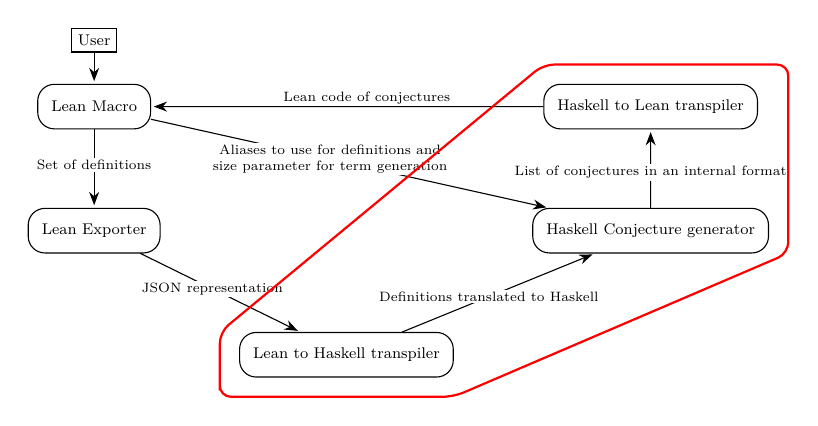
\begin{tikzpicture}[font=\footnotesize, ->, >={Stealth[sep]}, scale=0.7, every node/.style={scale=0.7}]
    \tikzstyle{module} = [rectangle, draw, rounded corners=6, inner sep=7, minimum height=23]
    \tikzstyle{desc} = [pos=0.45, fill=white, font=\scriptsize, align=center, inner sep=1]

    \node[draw]                          (us)  {User};
    \node[module, below      =0.4 of us] (lm)  {Lean Macro};
    \node[module, below      =of lm]     (ex)  {Lean Exporter};
    \node[module, below right=of ex]     (l2h) {Lean to Haskell transpiler};
    \node[module, above right=of l2h]    (cg)  {Haskell Conjecture generator};
    \node[module, above      =of cg]     (h2l) {Haskell to Lean transpiler};

    \draw (us)  -- (lm);
    \draw (lm)  -- (cg)  node[desc]        {Aliases to use for definitions and \\ size parameter for term generation};
    \draw (lm)  -- (ex)  node[desc]        {Set of definitions};
    \draw (ex)  -- (l2h) node[desc]        {JSON representation};
    \draw (l2h) -- (cg)  node[desc]        {Definitions translated to Haskell};
    \draw (cg)  -- (h2l) node[desc]        {List of conjectures in an internal format};
    \draw (h2l) -- (lm)  node[desc, above,fill=none] {Lean code of conjectures};

    \pause
    \draw[draw=gray, rounded corners, thick, draw=red, -]
      ([xshift=1em, yshift=1em]h2l.north east) -|
      ([xshift=1em]cg.south east) --
      ([yshift=-1em]l2h.south east) -|
      ([xshift=-1em, yshift=-1em]l2h.south west) -|
      ([xshift=-1em]l2h.north west) --
      ([yshift=1em]h2l.north west) --
      ([xshift=1em, yshift=1em]h2l.north east);
  \end{tikzpicture}
\end{figure}
\end{frame}
 % Kiren
% ~ 5 min
% An important piece of the puzzle is that Lean is very extensible.
% We can define new arbitrary syntax and then provide a function that elaborates its semantics.
% So here we see the keyword to do just that.
% We define a new elaborator for a command, which is basically the top level object in Lean files.
% ~~~~~~~~~~
% The syntax is defined to be the literal character sequence hash pisa.
% Followed by an optional number and a list of one or more identifiers.
% I've omited the elaboration definition for brevity
% ~~~~~~~~~~
% What we instead are interested in is the ability to associate a language server code action with our command.
% We can add an attribute to a CommandCodeAction definition to do this.
% As seen here
% ~~~~~~~~~~
% The function can then return any language server protocol message
% In this case we can provide a quickfix suggestion that lets the user insert the conjectures we generate.
% As you just saw in the demo.
% But to generate those we need more information.
% ~~~~~~~~~~
% This is provided by arguments to the code action.
% Specifically the snapshot contains the state of the Lean evaluator at this point in time.
% And the node is our syntax node, where we can obtain the number and identifiers
% ~~~~~~~~~~
% That information is sufficient for our exporter.
% The following is an example definition of a Boolean type
% And functions representing disjunctinos of two and three Boolean values respectively.
% Lastly an invocation of our macro.
% ~~~~~~~~~~
% However, the namespacing is an important detail here
% Within it the definitions are implicitly prefixed
% But writing the full names get rather wordy.
% When generating conjectures we want to preserve the provided identifiers.
% ~~~~~~~~~~
% Therefore the header of our export constitute a maping between fully qualified identifiers and the ones provided.
% Aditionally, this informs the conjecture generator what definitions were provided.
% ~~~~~~~~~~
% This is relevant as they likely are not the only definitions exported.
% As in this example where or3 is defined through the regular or.
% When translating the code, the former will not work without also exporting the latter.
% However, we don't want to provide conjectures involving all transitive definitions.
% ~~~~~~~~~~
% As previously mentioned we can retrive definitions from the snapshot given to the code action.
% This expression would be resolving the definition of or3
% ~~~~~~~~~~
% The result looks something like this.
% The details are not important here.
% But we can see references to the `or` function
% Practically all definitions in Lean are available as typed lambda expressions similar to this one.
% For the provided identifiers and all their transitive dependencies to be exported
% we serialize these expressions along with some additional information to JSON


\begin{frame}[fragile]{Macro} % Kiren
  \frametitle<1-2>{Macro: Definition}
  \frametitle<3->{Macro: Code Action}

  \begin{overprint}
  \onslide<1>
    \begin{LeanCodeHL}
      ˹‹˺elab˹›˺ "#pisa" n:(num)? is:(ident)+ ˹‹˺: command˹›˺ => ˹$…$˺
    \end{LeanCodeHL}
  \onslide<2>
    \begin{LeanCodeHL}
      elab ˹‹˺"#pisa" n:(num)? is:(ident)+˹›˺ : command => ˹$…$˺
    \end{LeanCodeHL}
  \onslide<3->
    \begin{LeanCodeHL}
      elab "#pisa" n:(num)? is:(ident)+ : command => ˹$…$˺
    \end{LeanCodeHL}
  \end{overprint}

  \begin{overprint}
    \onslide<3>
    \begin{LeanCodeHL}
      ˹‹˺@[command_code_action «#pisa»]˹›˺
      def insertConjectures : ˹‹˺CommandCodeAction˹›˺ :=
    \end{LeanCodeHL}

    \onslide<4->
    \begin{LeanCodeHL}
      @[command_code_action «#pisa»]
      def insertConjectures : CommandCodeAction :=
    \end{LeanCodeHL}
  \end{overprint}


  \begin{overprint}
    \onslide<4>
    \begin{LeanCodeHL}
      ˹˺  λ _ snapshot _ node => do
          ˹$…$˺
          return {
            ˹‹˺title := "Insert conjectures"˹›˺,
            ˹‹˺kind? := "quickfix"˹›˺,
            ˹‹˺edit? :=˹›˺ some <| .ofTextDocumentEdit {
              textDocument := ⟨uri, none⟩
              edits := #[ {
                range := text.utf8RangeToLspRange range,
                ˹‹˺newText := conjecturesText˹›˺,
              } ],
            }
          }
    \end{LeanCodeHL}

    \onslide<5>
    \begin{LeanCodeHL}
      ˹‹˺  λ _ snapshot _ node =>˹›˺ do
          ˹$…$˺
          return {
            title := "Insert conjectures",
            kind? := "quickfix",
            edit? := some <| .ofTextDocumentEdit {
              textDocument := ⟨uri, none⟩
              edits := #[ {
                range := text.utf8RangeToLspRange range,
                newText := conjecturesText
              } ]
            }
          }
    \end{LeanCodeHL}
  \end{overprint}
\end{frame}

\begin{frame}[fragile]{Exporter} % Kiren
  \frametitle<1>{Exporter: Example Code}
  \frametitle<2>{Exporter: Namespaces}
  \frametitle<3>{Exporter: Headers}
  \frametitle<4->{Exporter: Resolving definitions}

  \begin{overprint}
    \onslide<1,4->
      \begin{LeanCodeHL}
        ˹‹˺namespace ˹\tikzmark{exstrt}˺Example˹\tikzmark{exend}˺
        inductive B where | t : B | f : B
        def or˹\tikzmark{ordef}˺ : B → B → B := λ
          | .t, _ => .t
          | .f, b => b

        def or3˹\tikzmark{3def}˺ (a b c : B) : B := ˹\tikzmark{orref}˺or (or a b) c
      \end{LeanCodeHL}
    \onslide<2>
      \begin{LeanCodeHL}
        namespace ˹\tikzmark{exstrt}˺Example˹\tikzmark{exend}˺
        ˹‹˺inductive ˹›˺Example.˹‹˺B where | t : B | f : B
        def ˹›˺Example.˹‹˺or : B → B → B := λ
          | .t, _ => .t
          | .f, b => b

        def ˹›˺Example.˹‹˺or3 (a b c : B) : B := or (or a b) c
      \end{LeanCodeHL}
    \onslide<3>
      % \begin{minted}[escapeinside=˹˺,autogobble]{bash}
      %   pisa --size 4
      % \end{minted}
      \begin{JsonCode}
        [ ["Example.B", "B"]
        , ["Example.B.t", "B.t"]
        , ["Example.or3", "or3"]
        ]
      \end{JsonCode}
  \end{overprint}
  \begin{overprint}
    \onslide<1,4->
      \begin{LeanCodeHL}
        ˹‹˺#pisa 4 B B.t ˹\tikzmark{3ref}˺or3
      \end{LeanCodeHL}
    \onslide<2-3>
      \begin{LeanCodeHL}
        ˹‹˺#pisa 4 ˹›˺Example.˹‹˺B ˹›˺Example.˹‹˺B.t ˹›˺Example.˹‹˺or3
      \end{LeanCodeHL}
  \end{overprint}

  \begin{overprint}
    \onslide<5>
      \rule{\linewidth}{0.4pt}

      \begin{LeanCode}[frame=none, fontsize=\normalsize]
        snapshot.cmdState.env.find? `Example.or3
      \end{LeanCode}
  \end{overprint}

  \begin{overprint}
    \onslide<4->
    
\begin{tikzpicture}[overlay, remember picture, very thick, red!60, ->, >={Stealth[sep]}]
      \draw ([yshift=0.5em]pic cs:orref) -- (pic cs:ordef);
      \draw ([yshift=0.5em]pic cs:3ref) -- (pic cs:3def);
    \end{tikzpicture}

    \onslide<2>
    \begin{tikzpicture}[overlay, remember picture, >={Stealth[sep]}]
      \draw[blue!60,decorate,decoration={snake,amplitude=.1ex,segment length=.4ex}] ([yshift=-.5ex]pic cs:exstrt)--([yshift=-.5ex]pic cs:exend);
    \end{tikzpicture}
  \end{overprint}
  % \begin{itemize}
  %   \item Fetch dependencies of roots
  %   \item Convert to JSON
  % \end{itemize}
\end{frame}

\begin{frame}[fragile]{Exporter: ConstantInfo} % Kiren
  \begin{LeanCode}[frame=none]
    ConstantInfo.defnInfo {
      value := mkLambda `a .default (.const `Example.B [])
            <| mkLambda `b .default (.const `Example.B [])
            <| mkLambda `c .default (.const `Example.B [])
            <| .app (.app (.const ˹\tikzmark{mstrt}˺`Example.or˹\tikzmark{mend}˺ [])
                (.app (.app (.const `Example.or [])
                  (.bvar 2)) (.bvar 1)))
                (.bvar 0),
      type := mkForall `a .default (.const `Example.B [])
           <| mkForall `b .default (.const `Example.B [])
           <| mkForall `c .default (.const `Example.B [])
           <| .const `Example.B [],
      safety := .safe
      name := `Example.or3,
      levelParams := [],
      hints := .regular 2,
      all := [`Example.or3],
    }
  \end{LeanCode}
  \begin{tikzpicture}[overlay, remember picture, >={Stealth[sep]}]
    \draw[blue!60,decorate,decoration={snake,amplitude=.1ex,segment length=.4ex}] ([yshift=-.5ex]pic cs:mstrt)--([yshift=-.5ex]pic cs:mend);
  \end{tikzpicture}
\end{frame}

% {"defnInfo":
%  {"val":
%   {"value":
%    {"lam":
%     {"body":
%      {"lam":
%       {"body":
%        {"lam":
%         {"body":
%          {"app":
%           {"fn":
%            {"app":
%             {"fn": {"const": {"us": [], "declName": "Example.or"}},
%              "arg":
%              {"app":
%               {"fn":
%                {"app": {"fn": {"const": {"us": [], "declName": "Example.or"}}, "arg": {"bvar": {"deBruijnIndex": 2}}}},
%                "arg": {"bvar": {"deBruijnIndex": 1}}}}}},
%            "arg": {"bvar": {"deBruijnIndex": 0}}}},
%          "binderType": {"const": {"us": [], "declName": "Example.B"}},
%          "binderName": "c",
%          "binderInfo": "default"}},
%        "binderType": {"const": {"us": [], "declName": "Example.B"}},
%        "binderName": "b",
%        "binderInfo": "default"}},
%      "binderType": {"const": {"us": [], "declName": "Example.B"}},
%      "binderName": "a",
%      "binderInfo": "default"}},
%    "type":
%    {"forallE":
%     {"body":
%      {"forallE":
%       {"body":
%        {"forallE":
%         {"body": {"const": {"us": [], "declName": "Example.B"}},
%          "binderType": {"const": {"us": [], "declName": "Example.B"}},
%          "binderName": "c",
%          "binderInfo": "default"}},
%        "binderType": {"const": {"us": [], "declName": "Example.B"}},
%        "binderName": "b",
%        "binderInfo": "default"}},
%      "binderType": {"const": {"us": [], "declName": "Example.B"}},
%      "binderName": "a",
%      "binderInfo": "default"}},
%    "safety": "safe",
%    "name": "Example.or3",
%    "levelParams": [],
%    "hints": {"regular": 2},
%    "all": ["Example.or3"]}}}
 % Kiren
% ~2 min
% And that's that for the lean part so far.
% The exported data is now piped to the haskell executable and deserialized.
% This is where the main focus of our work happens.
% - Transpiling the Lean code to Haskell
% ~~~~~~~~
% There are two aspects to the transpilation that are handled a bit differently.
% Data types and their constructors for one
% And second, other definitions, mainly functions.
% ~~~~~~~~
% For data types there is a pretty straight forward corespondence between the languages
% as is demonstrated by this list-like data type.
% This is however somewhat fragile.
% In Haskell types and values live in two separate worlds,
% whereas in Lean types can depend regular values and are themselves regular values
% But for the scope of our tool, this difference is not accounted for.
% ~~~~~~~~
% The actual exported representation is more akin to this snipet.
% The important difference here is that the variable alpha is not shared between the definitions
% ~~~~~~~~
% So here's the same definition showcasing their independence
% But in the generated Haskell code this is not permitted
% So first we must homonogize these definitons by renaming and removing the type variable
% ~~~~~~~~
% When that is done, we simply have to be able to translate these type signatures
% Which happened to be pretty straight forward.
% ~~~~~~~~
% Finally, to help the conjecture generator abstractly represent arbitrary polymophism
% we have replace the type variable with a specific type called `Poly`
% What proved to not be as straight forward as this is translating regular definitions.

\begin{frame}{Lean to Haskell Transpiler} % Kiren
\begin{figure}
  \centering
  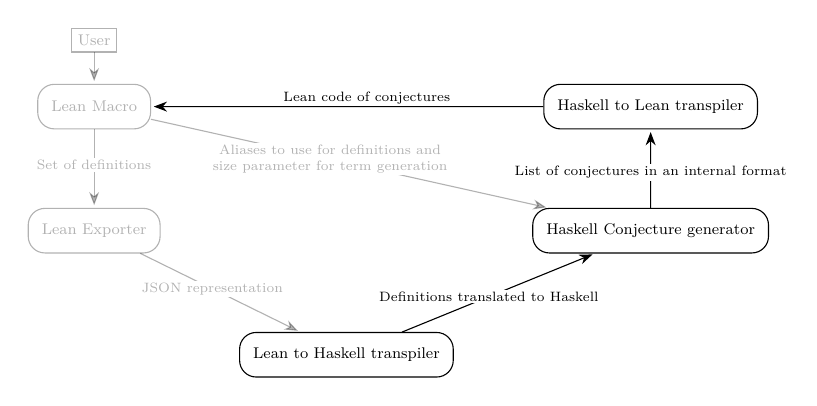
\begin{tikzpicture}[font=\footnotesize, ->, >={Stealth[sep]}, scale=0.7, every node/.style={scale=0.7}]
    \tikzstyle{module} = [rectangle, draw, rounded corners=6, inner sep=7, minimum height=23]
    \tikzstyle{desc} = [pos=0.45, fill=white, font=\scriptsize, align=center, inner sep=1]
    \tikzstyle{fesc} = [text opacity= 0.3, fill opacity=1, desc]

    \fade
    \node[draw]                          (us)  {User};
    \node[module, below      =0.4 of us] (lm)  {Lean Macro};
    \node[module, below      =of lm]     (ex)  {Lean Exporter};
    \unfade
    \node[module, below right=of ex]     (l2h) {Lean to Haskell transpiler};
    \node[module, above right=of l2h]    (cg)  {Haskell Conjecture generator};
    \node[module, above      =of cg]     (h2l) {Haskell to Lean transpiler};

    \fade
    \draw (us)  -- (lm);
    \draw (lm)  -- (cg)  node[fesc]        {Aliases to use for definitions and \\ size parameter for term generation};
    \draw (lm)  -- (ex)  node[fesc]        {Set of definitions};
    \draw (ex)  -- (l2h) node[fesc]        {JSON representation};
    \unfade
    \draw (l2h) -- (cg)  node[desc]        {Definitions translated to Haskell};
    \draw (cg)  -- (h2l) node[desc]        {List of conjectures in an internal format};
    \draw (h2l) -- (lm)  node[desc, above] {Lean code of conjectures};
  \end{tikzpicture}
\end{figure}
\end{frame}

\begin{frame}{Lean to Haskell Transpiler} % Kiren
  Two aspects

  \begin{itemize}
  \item Data types \& Constructors
  \item Definitions: Functions
  \end{itemize}

\end{frame}

\begin{frame}[fragile]{Lean to Haskell Transpiler: Data types \& Constructors} % Kiren
  % \begin{LeanCode}
  %   inductive B where | t :  B | f :  B
  % \end{LeanCode}
  % \begin{HaskellCode}
  %   data      B where ; T :: B ; F :: B
  % \end{HaskellCode}

  \begin{overprint}
    \onslide<1-2>
    \begin{columns}[T]
      \begin{column}{.48\textwidth}
        \begin{LeanCode}
          inductive L α
            where
            | Nil : L α
            | Cons : α → L α → L α
        \end{LeanCode}
        \centering
        Lean version
      \end{column}
      \begin{column}{.48\textwidth}
        \begin{HaskellCode}[fontsize=\small]
          data L α
            where
            Nil :: L α
            Cons :: α -> L α -> L α
        \end{HaskellCode}
        \centering
        Haskell version
      \end{column}
    \end{columns}
    \onslide<3-4>
    \begin{columns}[T]
      \begin{column}{.48\textwidth}
        \begin{LeanCode}
          inductive L : Type → Type
            where
            | Nil : L β
            | Cons : γ → L γ → L γ
        \end{LeanCode}
        \centering
        Lean version
      \end{column}
      \begin{column}{.48\textwidth}
        \begin{HaskellCode}[fontsize=\small]
          data L α
            where
            Nil :: L α
            Cons :: α -> L α -> L α
        \end{HaskellCode}
        \centering
        Haskell version
      \end{column}
    \end{columns}
    \onslide<5>
    \begin{columns}[T]
      \begin{column}{.48\textwidth}
        \begin{LeanCode}
          inductive L : Type → Type
            where
            | Nil : L β
            | Cons : γ → L γ → L γ
        \end{LeanCode}
        \centering
        Lean version
      \end{column}
      \begin{column}{.48\textwidth}
        \begin{HaskellCode}[fontsize=\small]
          data L Poly where
            Nil :: L Poly
            Cons :: Poly -> L Poly
                         -> L Poly
        \end{HaskellCode}
        \centering
        Haskell version
      \end{column}
    \end{columns}
  \end{overprint}

  \vspace{1cm}
  \begin{columns}[T]
    \begin{column}{.65\textwidth}
  \begin{overprint}
    \onslide<2>
    \begin{LeanCode}
      L := Type → Type
      L.Nil := (α : Type) → L α
      L.Cons := (α : Type) → α → L α → L α
    \end{LeanCode}
    \onslide<3>
    \begin{LeanCode}
      L := Type → Type
      L.Nil := (β : Type) → L β
      L.Cons := (γ : Type) → γ → L γ → L γ
    \end{LeanCode}
    \onslide<4->
    \begin{LeanCode}
      L := (α : Type) → Type
      L.Nil := L α
      L.Cons := α → L α → L α
    \end{LeanCode}
  \end{overprint}
      \end{column}
    \end{columns}
  \bigskip
  \begin{overprint}
    \onslide<2-3>
    \begin{center}
      Exported representation
    \end{center}
  \end{overprint}
\end{frame}

\begin{frame}[allowframebreaks,fragile]{Lean to Haskell Transpiler: Functions} % Pingu
  Intermediate representation used by Lean

  % So, a question that arises when using lean is how it evaluates expressions in the editor.
  % Short answer, using an IR that gets converted to C code, and is then evaluated.
  % What if, you can export the first iteration of this IR?
  % Turns out, you can

  \framebreak
  \begin{columns}[T]
    \begin{column}{.48\textwidth}
      \begin{LeanCode}
        inductive B where
          | t : B
          | f : B

        def not (b : B) : B :=
          match b with
          | .t => .f
          | .f => .t
      \end{LeanCode}
      \centering
      Lean version
    \end{column}
    \begin{column}{.48\textwidth}
      \begin{LeanIR}
        def not (x_1 : u8) : u8 :=
          case x_1 : u8 of
          B.t →
            let x_2 : u8 := 1;
            ret x_2
          B.f →
            let x_3 : u8 := 0;
            ret x_3
      \end{LeanIR}
      \centering
      IR version
    \end{column}
  \end{columns}

  % Here, we can see an example of the conversion between the Lean code and IR for the function not
  % It is quite similar, but worth noting is that the Boolean has been converted into an number, representing the index it held in the enum.
  % The IR tries to do these optimizations, even in the first iteration, since they allow for leaner (haha) code.

  \framebreak
  \begin{LeanCode}
  inductive L (α : Type) where
    | Nil : L α
    | Cons : α → L α → L α

  def append {α : Type} (xs : L α) (ys : L α) : (L α) :=
    match xs with
    | .Nil => ys
    | .Cons a as => .Cons a (append as ys)
  \end{LeanCode}

  % So what if, we have a more complicated example, such as append for lists.
  % There is polymorphism, and recursion in this, how does the IR handle it?

  \framebreak

  \begin{minted}[frame=single,autogobble,fontsize=\tiny]{Lean4}
  def append._rarg (x_1 : obj) (x_2 : @& obj) : obj :=
    case x_1 : obj of
    L.Nil →
      inc x_2;
      ret x_2
    L.Cons →
      let x_3 : u8 := isShared x_1;
      case x_3 : u8 of
      Bool.false →
        let x_4 : obj := proj[1] x_1;
        let x_5 : obj := append._rarg x_4 x_2;
        set x_1[1] := x_5;
        ret x_1
      Bool.true →
        let x_6 : obj := proj[0] x_1;
        let x_7 : obj := proj[1] x_1;
        inc x_7;
        inc x_6;
        dec x_1;
        let x_8 : obj := append._rarg x_7 x_2;
        let x_9 : obj := ctor_1[L.Cons] x_6 x_8;
        ret x_9
  def append (x_1 : ◾) : obj :=
    let x_2 : obj := pap append._rarg._boxed;
    ret x_2
  def append._rarg._boxed (x_1 : obj) (x_2 : obj) : obj :=
    let x_3 : obj := append._rarg x_1 x_2;
    dec x_2;
    ret x_3
  \end{minted}

  % The append function is ''just`` 2 lines.
  % But what is this black box?
  % And how does the _rarg work?
  % Well, the box is to allow for partially applied functions in a special way, and is named irrelevant.
  % It is done to allow for the boxing aspect, since the IR is based on Lambda RC which allows for mutable data.
  % And the actually applied values will be of the object type

  \framebreak

  What about values then?

  % Values are how IR handles, and for most of the types used, will usually either become objects, or enums.

  \framebreak

  \begin{HaskellCode}
    data Object = Object { rc :: Int, tag :: Natural }

    data Val
      = Unsigned Natural
      | ** ...**
      | VCtor { o :: Object, vs :: [Val] }

    fromValPoly :: Val -> Poly
    fromValPoly = \case
      Unsigned a -> Poly a

    toValPoly :: Poly -> Val
    toValPoly (Poly a) = Unsigned a
  \end{HaskellCode}

  % Here we can see the encoding of the different values, but since we need to be able to autogenerate the datatypes explained by Erik earlier, the Poly type was introduced to handle the case for conversion to naturals here.

  \framebreak

  \begin{HaskellCode}
    data L where
      Nil  :: L
      Cons :: Poly -> L -> L

    toValL :: L -> Val
    toValL = \a -> case a of
      Nil -> VCtor (Object 1 0) []
      Cons b c ->
        VCtor (Object 1 1) [toValPoly b, toValL c]

    fromValL :: Val -> L
    fromValL = \(a :: Val) -> case a of
      VCtor (Object _ 0) [] -> Nil
      VCtor (Object _ 1) [b, c] ->
        Cons (fromValPoly b) (fromValL c)
  \end{HaskellCode}

  % So each datatype that we introduce will have to create two functions.
  % One from Val and one to Val.
  % In the case of Lists, we utilize the Poly type to make it monomorphic.

\end{frame}

\begin{frame}[allowframebreaks,fragile]{Conjecture generation} % Pingu
  Get signatures of the roots

  Apply QuickSpec \& RoughSpec

  % So, we have the roots, as given by the user, and we have generated code to evaluate them.
  % Time to plop them into a list for QuickSpec and RoughSpec to generate conjectures on.
  % The signatures will be the name, and how to call them.
  % QuickSpec and RoughSpec will then create different combinations of the specified signatures, and test if they hold up.
  % If a case fails, that is tossed, otherwise they are kept as potential laws and presented to user.

  \pagebreak

  \begin{HaskellCode}
  environment :: Map Name Decl
  environment = fromList [**...**]

  append = FDecl {**...**}

  sigs :: [Sig]
  sigs =
    [ monoType ((Proxy :: Proxy L))
    , con "append"
        (\ a b -> fromValL
          (eval append environment
            [toValL a, toValL b]
          )
        )
    ]
  \end{HaskellCode}

  \pagebreak

  \begin{minted}[frame=single, autogobble]{Output}
  == Laws ==
    1. append (append x y) z = append x (append y z)
  \end{minted}

  % Here we can see an example of what would be expected if only the append function is supplied.
  % And this is the associativity law, which would be expected.

\end{frame}

\begin{frame}[allowframebreaks,fragile]{Reverse translation} % Pingu
  The names of functions can be preserved

  The types need to be kept in a map

  \pagebreak

  \begin{minted}[frame=single, autogobble, fontsize=\footnotesize]{Lean}
  (x y z : T0'L) : append (append x y) z = append x (append y z)
  \end{minted}
  \fade
  \begin{minted}[frame=single, autogobble, fontsize=\footnotesize]{Lean}
  (x y z : L α)  : append (append x y) z = append x (append y z)
  \end{minted}

  \pagebreak

  \fade
  \begin{minted}[frame=single, autogobble, fontsize=\footnotesize]{Lean}
  (x y z : T0'L) : append (append x y) z = append x (append y z)
  \end{minted}
  \unfade
  \begin{minted}[frame=single, autogobble, fontsize=\footnotesize]{Lean}
  (x y z : L α)  : append (append x y) z = append x (append y z)
  \end{minted}

  % Worth of note is that the names of the functions will not always match up with the ones that can be seen for the user in the editor.
  % But when constructing the signatures, replacement names can be provided, which override the internal names.
  % That is great for us, but the names of types are not.
  % So a mapping between the internal Haskell name and the Lean name is kept for reversing it when sent back to the Lean part.
\end{frame}
 % Pingu
\begin{frame}[fragile]{Macro} % Kiren
  \begin{figure}
    \centering
    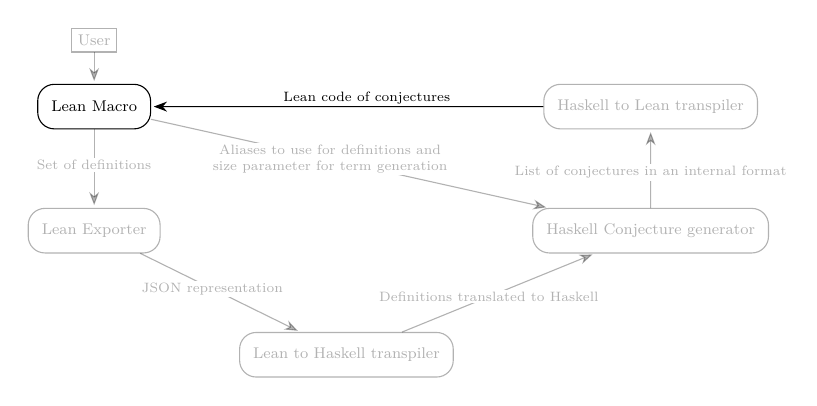
\begin{tikzpicture}[font=\footnotesize, ->, >={Stealth[sep]}, scale=0.7, every node/.style={scale=0.7}]
      \tikzstyle{module} = [rectangle, draw, rounded corners=6, inner sep=7, minimum height=23]
      \tikzstyle{desc} = [pos=0.45, fill=white, font=\scriptsize, align=center, inner sep=1]
      \tikzstyle{fesc} = [text opacity= 0.3, fill opacity=1, desc]

      \fade
      \node[draw]                          (us)  {User};
      \unfade
      \node[module, below      =0.4 of us] (lm)  {Lean Macro};
      \fade
      \node[module, below      =of lm]     (ex)  {Lean Exporter};
      \node[module, below right=of ex]     (l2h) {Lean to Haskell transpiler};
      \node[module, above right=of l2h]    (cg)  {Haskell Conjecture generator};
      \node[module, above      =of cg]     (h2l) {Haskell to Lean transpiler};
      \unfade

      \fade
      \draw (us)  -- (lm);
      \draw (lm)  -- (cg)  node[fesc]        {Aliases to use for definitions and \\ size parameter for term generation};
      \draw (lm)  -- (ex)  node[fesc]        {Set of definitions};
      \draw (ex)  -- (l2h) node[fesc]        {JSON representation};
      \draw (l2h) -- (cg)  node[fesc]        {Definitions translated to Haskell};
      \draw (cg)  -- (h2l) node[fesc]        {List of conjectures in an internal format};
      \unfade
      \draw (h2l) -- (lm)  node[desc, above] {Lean code of conjectures};
    \end{tikzpicture}
  \end{figure}
  \smallskip
  \begin{LeanCode}
    let conjecturesText ← IO.spawn "pisa" =<< export is
  \end{LeanCode}
\end{frame}

\setbeamercovered{transparent}
\begin{frame}{Alternatives approaches} % Kiren
  \begin{itemize}[<+>]
    \item Instantiations of polymorphism
    \item Proof generation
    \item Proper translation using reductions
    \item Performance
    \item Plausible
  \end{itemize}
\end{frame}
 % Kiren

\end{document}
